%\documentclass[12pt,notitlepage]{article}
\documentclass[a4paper,12pt]{article}
\usepackage[utf8]{inputenc}
\usepackage{graphicx}
\usepackage{verbatim}
\usepackage{amsthm}
\usepackage{pdfpages}
\usepackage{amsmath}
\usepackage{enumerate} 

\usepackage{mathtools}
\DeclarePairedDelimiter\ceil{\lceil}{\rceil}
\DeclarePairedDelimiter\floor{\lfloor}{\rfloor}

\usepackage{hyperref}
%\usepackage[T1]{fontenc}
\usepackage{url}
\usepackage{lipsum}
\usepackage{array}
\usepackage{multirow}
\usepackage{float}
\usepackage{lscape}
\usepackage{colortbl}
\newcolumntype{P}[1]{>{\centering\arraybackslash}p{#1}}
\usepackage[nottoc,numbib]{tocbibind}
\usepackage{fancyhdr}
\usepackage{hhline}
\usepackage[printonlyused]{acronym}

\usepackage{tabularx}
\usepackage{tabulary}

%\usepackage{txfonts}
\usepackage{lipsum,etoolbox}% http://ctan.org/pkg/{lipsum,etoolbox}
\usepackage{caption}
\usepackage{subcaption}
\usepackage[normalem]{ulem}

\usepackage{algorithm}
\usepackage[noend]{algpseudocode}

\makeatletter
\def\BState{\State\hskip-\ALG@thistlm}
\makeatother

\usepackage{minted}

\definecolor{black}{RGB}{0,0,0}

\usepackage{fancyvrb}

\usepackage{geometry}
\geometry{
	a4paper,
	total={170mm,257mm},
	right=3cm,
	left=3.5cm,
	top=3cm,
	bottom=3cm
}


\usepackage{titlesec}
\usepackage{hyperref}
\titleclass{\subsubsubsection}{straight}[\subsection]

\newcounter{subsubsubsection}[subsubsection]
\renewcommand\thesubsubsubsection{\thesubsubsection.\arabic{subsubsubsection}}
\renewcommand\theparagraph{\thesubsubsubsection.\arabic{paragraph}} % optional; useful if paragraphs are to be numbered

\titleformat{\subsubsubsection}
{\normalfont\normalsize\bfseries}{\thesubsubsubsection}{1em}{}
\titlespacing*{\subsubsubsection}
{0pt}{3.25ex plus 1ex minus .2ex}{1.5ex plus .2ex}

\makeatletter
\renewcommand\paragraph{\@startsection{paragraph}{5}{\z@}%
	{3.25ex \@plus1ex \@minus.2ex}%
	{-1em}%
	{\normalfont\normalsize\bfseries}}
\renewcommand\subparagraph{\@startsection{subparagraph}{6}{\parindent}%
	{3.25ex \@plus1ex \@minus .2ex}%
	{-1em}%
	{\normalfont\normalsize\bfseries}}
\def\toclevel@subsubsubsection{4}
\def\toclevel@paragraph{5}
\def\toclevel@paragraph{6}
\def\l@subsubsubsection{\@dottedtocline{4}{7em}{4em}}
\def\l@paragraph{\@dottedtocline{5}{10em}{5em}}
\def\l@subparagraph{\@dottedtocline{6}{14em}{6em}}
\makeatother

\setlength\parindent{0pt}

\setcounter{secnumdepth}{4}
\setcounter{tocdepth}{4}

\newtheorem{dummy}{Dummy} %dummy for numbering purposes

\theoremstyle{definition}
\newtheorem{definition}[dummy]{Definition}
\newtheorem{example}[dummy]{Example}
\newtheorem{exercise}[dummy]{Exercise}
\newtheorem{remark}[dummy]{Remark}
\newtheorem{fact}[dummy]{Fact}
\newtheorem{ques}[dummy]{QUESTION}

\theoremstyle{plain}
\newtheorem{theorem}[dummy]{Theorem}
\newtheorem{proposition}[dummy]{Proposition}
\newtheorem{corollary}[dummy]{Corollary}
\newtheorem{lemma}[dummy]{Lemma}


\newcommand{\ttx}[1]{\texttt{#1}}

\newcommand{\biganglebracket}[1]{\left\langle #1 \right\rangle}
\newcommand{\bigbracket}[1]{\left( #1 \right)}
\newcommand{\bigsquarebracket}[1]{\left[ #1 \right]}
\newcommand{\bigcurlybracket}[1]{\left\{ #1 \right\}}
\newcommand{\bigfloorbracket}[1]{\left\lfloor #1 \right\rfloor}
\newcommand{\bigceilbracket}[1]{\left\lceil #1 \right\rceil}
\newcommand{\bigabs}[1]{\left| #1 \right|}
\newcommand{\bignorm}[1]{\left\| #1 \right\|}

\begin{document}
	\begin{titlepage}
			\begin{center}
				%		\large
				\textbf{NANYANG TECHNOLOGICAL UNIVERSITY}\\
				\vspace{1em}
				SEMESTER 1 EXAMINATION 2016-2017\\
				\vspace{1em}
				\textbf{MH1401/CY1401 - Algorithms and COmputing I}
			\end{center}
			\vspace{4.5em}
			
			\noindent August 2017 \hfill TIME ALLOWED: 30 MINUTES
			\vspace*{2em}
			
			\vbox{\hrule width\linewidth height 0.5pt}
			\vspace*{3em}
			
			\noindent\underline{INSTRUCTIONS TO CANDIDATES}
			\vspace*{1.5em}
			\begin{enumerate}
				\item This examination paper contains \textbf{FOUR (4)} questions and comprises \textbf{SIX (6)} printed pages.
				
				\item Answer \textbf{all} questions. The marks for each question are indicated at the beginning of each question.
				
				\item Answer each question beginning on a \textbf{FRESH} page of the answer book.
				
				\item This \textbf{IS NOT} and \textbf{OPEN BOOK} exam.
				
				\item This paper has been converted from the original MATLAB exam to a PYTHON exam. All questions are the property of Nanyang Technological University.
			\end{enumerate}
	\end{titlepage}

%\pagenumbering{roman}

%	\tableofcontents
	\newpage
	\pagenumbering{arabic}
	\setcounter{page}{2}
%	\addcontentsline{toc}{section}{Questions}

\hfill MH1401/CY1401\vspace*{0.5em}

\begin{ques}\hfill \textbf{(28 marks)}\\
	%		Kenneth had a little lamb\\
	%		Whose fleece was sheared by Lan\\
	%		She needed it for Bio lab\\
	%		But her experiment would not run
	\begin{enumerate}[(a)]
		\item Assume that an integer input \texttt{x} is given by a user. How do you check that \ttx{x} is a positive integer?
		
		\item Given a vector \ttx{vec} initialised as $[1, 0, 3, 0]$, what would be the result of the following command?\vspace*{1em}
		
		\texttt{any(vec) \&\& all(vec)}
		
		\item Given the matrix\begin{equation*}
		\text{\ttx{mat}} = \begin{pmatrix*}
		1 & 2 & 3\\4 & 5 & 6\\7 & 8 & 9
		\end{pmatrix*},
		\end{equation*}
		what is the result of the following command?\vspace*{1em}
		
		\texttt{np.sum(mat[0,2]*mat[0,:]))}
		
		\item Rewrite the following \texttt{if-elif} statement as a nested \texttt{if-else} statement that accomplishes exactly the same thing. Assume that \texttt{x} is an integer variable that has been initialised and the function \texttt{f(x,d)} is defined.
		\begin{verbatim}
		if x < -3 or x >= 3:
		    y=f(x,1)
		elif x > 0:
		    y=f(x,2)
		elif x < 0:
		    y=f(x,3)
		else:
		    y=f(x,4)
		\end{verbatim}
	\end{enumerate}
\end{ques}

\newpage

\hfill MH1401/CY1401\vspace*{0.5em}

\begin{ques}\hfill \textbf{(24 marks)}\vspace*{2em}\\
	%		Kenneth had a little lamb\\
	%		Whose fleece was sheared by Lan\\
	%		She needed it for Bio lab\\
	%		But her experiment would not run
	In Singapore, personal income tax rates for resident taxpayers are progressive. This means higher income earners pay a proportionately higher tax, with the current highest personal income tax rate at 20\%.
	
	\begin{enumerate}[(i)]
		\item Imagine a very simple tax system where a citizen pays an income tax rate with the rule from the table below.
		\begin{table}[H]
			\centering
			\begin{tabular}{|c|c|}
				\hline
				\textbf{Income} (in SGD) & \textbf{Tax rate}\\
				\hline
				$0$ to $20,000$ included & 0\%\\
				$20,001$ to $40,000$ included & 5\%\\
				$40,001$ to $100,000$ included & 10\%\\
				$100,001$ to $200,000$ included & 15\%\\
				more than $200,001$ & 20\%\\
				\hline
			\end{tabular}
		\end{table}
		For example, if a citizen has an income of $45,000$ SGD, he will be in the 10\% rate section, so he will pay $45,000\times 0.1 = 4,500$ SGD. Write a function \ttx{income\_tax} that will take as input the income of the citizen, and that will return the income tax amount he has to pay. Assume that the income value input is always an integer.
		
		
		\item In Singapore (and in many other countries), the rule is slightly more complex as the income is taxed in layers, with a higher tax rate applied to each successive layer. Using the same Table as before, a citizen will pay a 0\% tax rate for its first $20,000$ SGD, then a 5\% tax rate for the next $20,000$ SGD, then a 10\% tax rate for its next $60,000$ SGD, etc.
		
		For example, if a citizen has an income of $145,000$ SGD, the first $20,000$ SGD are taxed at a 0\% tax rate, then the next $20,000$ SGD are taxed at a 5\% tax rate, then the next $60,000$ SGD are taxed at a 10\% rate, and finally the remaining $45,000$ SGD are taxed at a 15\% rate. In total, he would have to pay $(20,000\times 0 + 20,000\times 0.05 + 60,000 \times 0.1 + 45,000\times 0.15) = 13,750$ SGD.
		
		Write again a function \ttx{income\_tax\_sg} that will take as input the income of the citizen, and that will return the income tax amount he has to pay for this new tax system. Assume that the income value input is always an integer.
	\end{enumerate}
\end{ques}

\newpage

\hfill MH1401/CY1401\vspace*{0.5em}

\begin{ques}\hfill \textbf{(24 marks)}\vspace*{2em}\\
	%		Kenneth had a little lamb\\
	%		Whose fleece was sheared by Lan\\
	%		She needed it for Bio lab\\
	%		But her experiment would not run
	Newton's method is a method for finding successively better approximations to the roots (or zeroes) of a real-valued function. It can be used to easily find a good approximation of the square root of a number $X\geq 0$. Let $R_1 > 0$ be a rather close approximation of $\sqrt{X}$, then $R_2 = \frac{1}{2}\bigbracket{\frac{R_1+X}{R_1}}$ offers an even better approximation of $\sqrt{X}$.
	
	\begin{enumerate}[(i)]
		\item Write a \textbf{recursive} function \ttx{newton\_sqrt(X,n)} that will return the $n$-th approximation of $\sqrt{X}$ using Newton's method (starting with $R_1 = 10$ as first approximation). As error check, the function returns $-1$ when $X$ is negative or when $n$ is not a positive integer.
		
		\item Assume that you have access to the function \ttx{newton\_sqrt(X,n)} described above. Write a function \ttx{newton\_sqrt\_approx(X,a)} that will output
		\begin{itemize}
			\item how many approximation steps are needed using Newton's method (starting with $R_1 = 10$ as first approximation), so that the distance between the approximation and the real $\sqrt{X}$ value is smaller of equal to $a$, and
			\item the corresponding distance value when the sufficiently close approximation is found.
		\end{itemize}
		Warning: note that the function outputs two values (by output, we mean that the function itself outputs the value, not just a printing on the screen). Hint: you can use the built-in functions \ttx{sqrt} and \ttx{absolute} in the \ttx{numpy} package in PYTHON.
	\end{enumerate}
\end{ques}

\newpage

\hfill MH1401/CY1401\vspace*{0.5em}

\begin{ques}\hfill \textbf{(24 marks)}\vspace*{2em}\\
	%		Kenneth had a little lamb\\
	%		Whose fleece was sheared by Lan\\
	%		She needed it for Bio lab\\
	%		But her experiment would not run
	The Tower of Hanoi is a well-known mathematical game. It consists of \textbf{three rods}, and a number of disks of different sizes which can slide onto any of the three rods. The puzzle starts with all the disks stacked in ascending order of size on the first rod, the smallest at the top, thus making a conical shape (see picture below). The objective of the puzzle is to move the entire stack to the third rod (only one disk can be moved at a time), obeying the following simple rules:
	\begin{itemize}
		\item Each move consists of taking the upper disk from one of the stacks and placing it on top of another stack, i.e. a disk can only be moved if it is the uppermost disk on a stack.
		
		\item No disk may be placed on top of a smaller disk.
	\end{itemize}
	
	\begin{figure}[H]
		\centering
		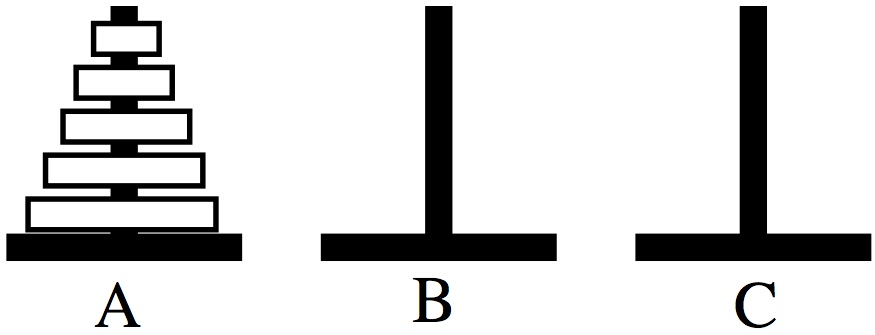
\includegraphics[scale=0.3]{TowersOfHanoiFigure.jpg}
	\end{figure}
	
	One can model this game in PYTHON by representing each rod by a vector (say \ttx{a} for first rod, \ttx{b} for second rod, \ttx{c} for third rod), and each disk by a value (a bigger disk is represented by a bigger value). The first element of a rod vector represents the closest disk to the base of the rod, then the second element of a rod vector represents the second closest disk to the base of the rod, etc. For example, with five disks, at the start of the game, \ttx{a} would be the vector $[5, 4, 3, 2, 1]$, while \ttx{b} and \ttx{c} would be empty vectors. If I move the top disk from the first rod to the third rod, then \ttx{a} would be the vector $[5,4,3,2]$, while \ttx{b} would be an empty vector and \ttx{c} would be the vector $[1]$.\vspace*{1em}
	
	\quad Note: Question No. 4 continues on page 6
	
	\newpage
	
	\hfill MH1401/CY1401\vspace*{0.5em}
	
	\begin{enumerate}[(i)]
		\item Implement a function \ttx{check\_move} that takes as input two rod vectors \ttx{x} and \ttx{y}. The function will check if moving the top disk of rod \ttx{x} to rod \ttx{y} is a valid move (according the game rules). Note that if rod \ttx{x} is empty, it is also considered an invalid move. If the move is invalid, the function will return the value $-1$. Otherwise, if the move is possible, the function will return $0$.
		
		\item Implement a function \ttx{check\_victory} that takes as input a rod vector \ttx{x}, and outputs the value $1$ if this rod contains all the disks (you can assume that the game contains $5$ disks in total). Otherwise, it outputs $0$.
		
		\item Assume that you have access to the functions \ttx{check\_move} and \ttx{check\_victory} described above. Implement a script that will ask a human player to input two rods' indexes \ttx{x} and \ttx{y} (you can assume that the player never inputs an error, the indexes always belong to $[1,2,3]$), check if the move from red \ttx{x} to rod \ttx{y} is valid, and execute this move if it is indeed a valid one. The script will then repeat the process until a victory is attained by the human player. (Hint: use a list or an array to store the three rods' vectors, so you can access them directly with indexes.)
	\end{enumerate}
\end{ques}

\end{document}